\startchapter{The Dark Higgs Model}
\label{chapter:dh_model}

The dark matter (DM) search presented in this thesis is motivated by and interpreted with the ``Dark Higgs" (DH) model \cite{Duerr2017}. The DH model predicts a mechanism for DM production from proton-proton collisions at the LHC by means of portal interactions with the dark sector. The dark sector, which is predicted as part of various BSM physics models, represents a collection of quantum fields and associated particles which are assumed to interact gravitationally, but which do not couple via any of the other known forces - electromagnetic, strong and weak - of the SM. Non-gravitational couplings between the dark sector and the SM proceed instead via one or more so-called ``portal mediators". 

In the DH model, the DM is a particle which belongs to the dark sector, and is produced from high-energy \(q\bar{q}\) collisions at the LHC via a hypothetical spin 1 vector boson portal mediator referred to as the \Zprime. The model introduces an additional Higgs boson in the dark sector called the ``Dark Higgs" (DH), which acts as a portal mediator by decaying to SM particles via a small mixing with the SM Higgs boson. 

Figure \ref{fig:Feynman_DH} shows three Feynman diagrams \textcolor{red}{(Note to Bob/self: may need to briefly introduce Feynman diagrams in ch. 1)} which illustrate some of the dominant modes by which the DH model could produce a measurable signature of DM production at the LHC. In all cases, the DM pair is produced via the \Zprime mediator, along with the emission of a DH boson \(s\), which decays to a pair of SM particles. 

\begin{figure}[hp]
	\centering
	\begin{subfigure}[t]{0.49\textwidth}
	\centering
	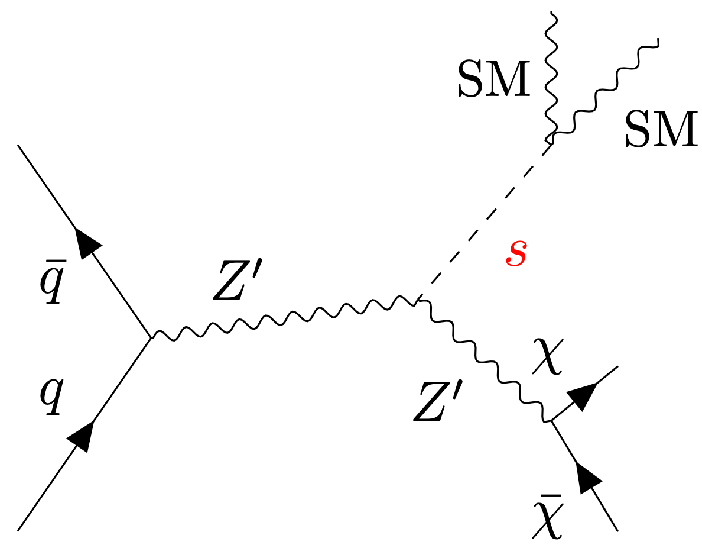
\includegraphics[width=0.95\textwidth]{Figures/2/Fey1.pdf}
%		\begin{tikzpicture}
%			\begin{feynman}
%
%		 		\vertex (a1);
%		 		\vertex[below=7em of a1] (b1);
%		 		\vertex at ($(a1)!0.5!(b1) + (1cm, 0)$) (c1); %z'
%		 		\vertex at ($(a1)!0.4!(b1) + (3cm, 0)$) (c2); %z'
%
%		 		\vertex[right=4cm of a1] (a2); % s
%		 		\vertex[below=5em of a2] (b2); % z'
%
%		 		\vertex at ($(c2) + (1.5cm, 0) + (0,-0.5cm)$) (a3);
%		 		\vertex[below=3em of a3] (b3);
%
%		 		\vertex at ($(a2) + (0, 1cm)$) (a4) ;
%		 		\vertex at ($(a2) + (0, 0.8cm) + (0.8cm, 0)$) (b4) ;
%
%		 		\diagram* {
%		 		  {[edges=fermion]
%		 		    (b1) -- [edge label=\(q\)]( c1) -- [edge label=\(\bar{q}\)](a1),
%		 		    (b3) -- [edge label=\(\bar{\chi}\)] (b2) -- [edge label=\(\chi\)]  (a3),
%		 		  },
%		 		  (c1) -- [boson, edge label=\(Z'\)] (c2),
%		 		  (a2) -- [scalar,edge label=\(\color{red} s\)] (c2) -- [boson, edge label'=\(Z'\)] (b2),
%		 		  (a4) -- [boson, edge label'={\small SM}] (a2) -- [boson, edge label'=\small{SM}] (b4),
%
%		 		};
%		 	\end{feynman}
%		 \end{tikzpicture}
	\caption{s-channel (DH and DM emitted from the \Zprime)}
	\end{subfigure}
		\begin{subfigure}[t]{0.45\textwidth}
	\centering
	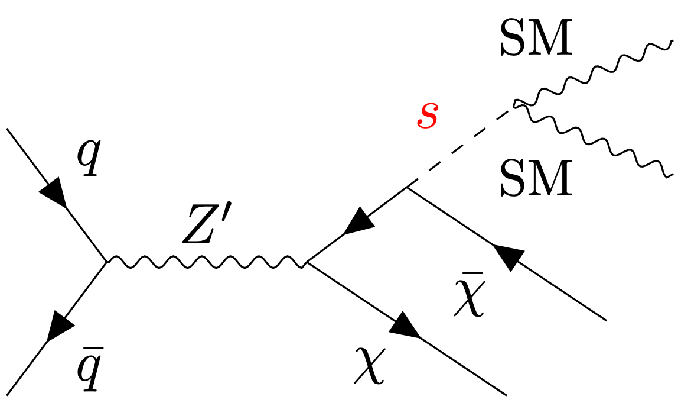
\includegraphics[width=0.95\textwidth]{Figures/2/Fey2.pdf}
%		\begin{tikzpicture}
%			\begin{feynman}
%
%		 		\vertex (b1);
%		 		\vertex at ($(b1) + (-0.75cm, 1cm)$) (a1); %q
%		 		\vertex at ($(b1) + (-0.75cm, -1cm)$) (a2); %qbar
%				\vertex at ($(b1) + (1.5cm, 0cm)$) (c1); %Z'
%				\vertex at ($(c1) + (1.5cm, -1cm)$) (d1); %chi
%				\vertex at ($(c1) + (0.75cm, 0.56cm)$) (d2); %chi
%				\vertex at ($(d2) + (1.5cm, -1cm)$) (d3); %chibar
%				\vertex at ($(d2) + (0.8cm, 0.6cm)$) (e1); %s
%				\vertex at ($(e1) + (1.2cm, 0.5cm)$) (f1); %W
%				\vertex at ($(e1) + (1.2cm, -0.5cm)$) (f2); %W
%				
%				\diagram* {
%				 (a1) -- [fermion, edge label=\(q\)](b1) -- [fermion, edge label=\(\bar{q}\)](a2),
%				 (b1) -- [boson, edge label=\(Z'\)] (c1),
%				 (d3) -- [fermion, edge label=\(\bar{\chi}\)](d2) -- [fermion](c1) -- [fermion, edge label'=\(\chi\)](d1),
%				 (d2) -- [scalar, edge label=\(\color{red} s\)] (e1),
%				 (f1) -- [boson, edge label'={\small SM}](e1) -- [boson, edge label'={\small SM}](f2),
%		 		};
%		 	\end{feynman}
%		 \end{tikzpicture}
	\caption{s-channel (DM emitted from the \Zprime, DH emitted from the DM)}
	\end{subfigure}
	\begin{subfigure}[t]{.42\textwidth}
	\centering
	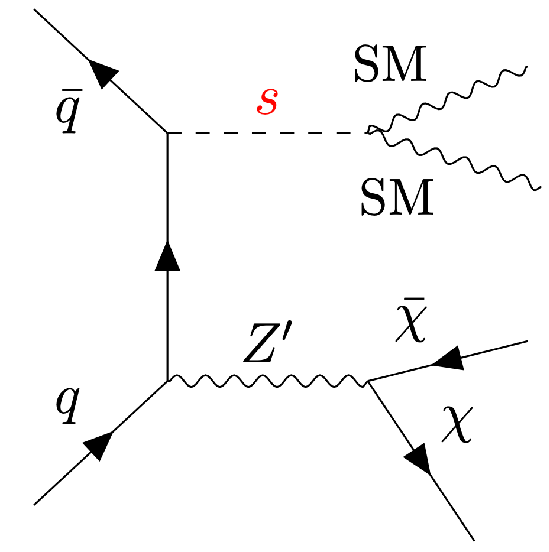
\includegraphics[width=0.95\textwidth]{Figures/2/Fey3.pdf}
%		 \begin{tikzpicture}
%		 	\begin{feynman}
%		 		\vertex (a1); %qbar
%		 		\vertex[below=9em of a1] (b1); %q
%				\vertex at ($(a1)!0.25!(b1) + (1cm, 0)$) (b5); %s
%		 		\vertex at ($(a1)!0.75!(b1) + (1cm, 0)$) (c1); %z'
%		 		\vertex at ($(c1) + (1.5cm, 0) + (0,0)$) (c2); %z'
%
%	         		\vertex[right=1.5cm of b5] (a2); % s
%		 		\vertex[below=2em of a2] (b2); % z'
%
%		 		\vertex at ($(c2) + (0.8cm, 0) + (0,-1.2cm)$) (a3);
%		 		\vertex at ($(c2) + (1.2cm, 0) + (0,0.3cm)$) (b3);
%
%		 		\vertex at ($(a2) + (1.2, 0.5cm)$) (a4) ;
%		 		\vertex at ($(a2) + (0, -0.4cm) + (1.3cm, 0)$) (b4) ;
%
%		 		\diagram* {
%		 		  {[edges=fermion, very thick]
%		 		    (b1) -- [edge label=\(q\)]( c1) -- (b5) -- [edge label=\(\bar{q}\)](a1),
%		 		    (b3) -- [edge label'=\(\bar{\chi}\)] (c2),
%		 		    (c2) -- [edge label=\(\chi\)]  (a3),
%		 		  },
%		 		  {[very thick]
%		 		  (c1) -- [boson, edge label=\(Z'\)] (c2),
%		 		  (b5) -- [scalar,edge label=\(\color{red} s\)] (a2),
%		 		  (a4) -- [boson, edge label'={\small SM}] (a2) -- [boson, edge label'={\small SM}] (b4),
%	         		  }
%		 		};
%		 	\end{feynman}
%		 \end{tikzpicture}
	\caption{t-channel (DH radiated off \(q\), DM emitted from the \Zprime)}
	\end{subfigure}
	\caption{The most contributing Feynman diagrams for DM production at the LHC by means of the DH model}
	\label{fig:Feynman_DH}
\end{figure}


\section{Theoretical Motivation for the Dark Higgs Model}

Given that the particles of the SM acquire mass via their interaction with the Higgs field \cite{HiggsTheory1,HiggsTheory2,HiggsTheory3}, the hypothetical ``Dark Higgs" field - and its associated particle the DH boson - is motivated by the need to likewise generate masses of particles in the dark sector. Furthermore, by virtue of its role as a portal mediator between dark sector and SM particles, the DH boson opens up a new mechanism by which processes of annihilation and creation between DM and SM particles could take place in the early Universe. According to the thermal freeze-out hypothesis discussed in Chapter 1, these creation and annihilation processes would have produced thermal equilibrium between SM particles and the dark sector in the early Universe \cite{DM_earlyUniverse}, which set the DM relic abundance observed in the Universe today. 

\subsection{Experimental Constraints on Direct DM Annihilation to SM Particles} 

This section presents the current experimental constraints on models which predict the establishment of the observed relic abundance of DM via direct creation and annihilation processes between DM and SM particles. This is followed by a discussion of how the experimental constraints can be relaxed by the introduction of a new annihilation channel \(\chi\chi \rightarrow ss\) followed by decays of \(s\) to SM particles, which arises naturally if particles in the dark sector obtain their mass by interacting with a new Higgs field in the dark sector.   


As discussed above, the hypothesized decay of the DH to SM particles would proceed via a small mixing between the DH and the SM Higgs boson. 

\begin{itemize}
\item Mixing between SM Higgs and dark sector Higgs.
\end{itemize}

\section{Model Description}
\begin{itemize}
\item Introduce it in the context of the wider class of dark sector models.
\item Describe the production mechanism, including leading Feynman diagrams.
\item Specify couplings to both SM and dark sector particles. 
\item Emphasize that $m_\chi>\frac{1}{2}\ms$ required to obtain signature in detector (otherwise $s\rightarrow\chi\chi$ decay would dominate).
\end{itemize}

\section{Search for the Dark Higgs Model at the LHC}

\begin{itemize}
\item Discussion of the model's signature in the ATLAS detector (boosted SM pair recoiling against \met), and why the boosted topology is unique compared with generic mono-X searches in which the `X' is produced via ISR.
\item Discussion of available search channels - mono-s(bb), mono-s(WW), mono-s(ZZ), mono-s(hh).
\begin{itemize}
\item Overview of existing searches for the Dark Higgs model - re-interpreted mono-h(bb), hadronic mono-s(WW). Could also mention ongoing dedicated mono-s(bb) search.
\item Identify the \ms regime in which the $s\rightarrow WW$ decay mode dominates in sensitivity.
\end{itemize}
\end{itemize}